\begin{subsection}{The \texttt{label} command}
One of the nicest features of \MP{} is that it relies on \TeX{} (or \LaTeX) to typeset labels within figures.  Almost all figures in technical documents are accompanied by labels which help clarify the situation for which the figure is assisting to illustrate.  Such labels may include anything from simple typesetting as in Figures \ref{fig:draw1}, \ref{fig:annulus2}, and \ref{fig:draw2} to typesetting function declarations and even axes labeling.

The \texttt{label} command requires two arguments\Dash a string to typeset and the point for which label is placed.  For example, the command \begin{center}\verb|label("A",(0,0));|\end{center} will place the letter ``A'' at the coordinate \texttt{(0,0)} and the box around this label is centered vertically and horizontally at this point.  Simple strings like \texttt{"A"} require no real typesetting to ensure that they appear properly in the figure.  However, many typeset strings in technical figures require the assistance of \TeX{} to properly display them.
\begin{figure}[hptb]
	\begin{center}\textattachfile[color={0 0 0},mimetype={text/plain}]{parabola.mp}{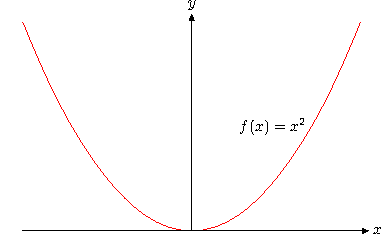
\includegraphics{parabola.mps}}\end{center}
	\caption{Labeling text}\label{fig:parabola}
\end{figure}
For example, Figure \ref{fig:parabola} is an example where typesetting is preferred.  That is, the axes labels and the function declaration look less than perfect if \TeX{} is not used.  For reasons such as this, \MP{} provides a way to \textit{escape} to \TeX{} in order to assist in typesetting the labels.  Therefore, instead of labeling the ``A'' as above, \begin{center}\verb|label(btex A etex,(0,0));|\end{center} provides a much nicer technique for typesetting the label.  The \texttt{btex\,...\,etex} block instructs \MP{} to process everything in between \texttt{btex} and \texttt{etex} using \TeX.  Therefore, the function declaration in Figure \ref{fig:parabola} is labeled using \begin{center}\verb|label(btex $f(x)=x^2$ etex,(|$a,b$\verb|));|\end{center} where \verb|(|$a,b$\verb|)| is the point for which the label is to be centered.

Since many \MP{} users prefer to typeset their labels using \LaTeX{} instead of plain \TeX, \MP{} provides a convenient method for accommodating this, done in the preamble of the \MP{} source file.  The following code ensures that the \verb|btex...etex| block escapes to \LaTeX{} (instead of plain \TeX) for text processing.
\begin{lstlisting}[xleftmargin=56bp]
verbatimtex
%&latex
\documentclass{minimal}
\begin{document}
etex
beginfig(|$n$|);
|\quad$\langle\mbox{\normalfont\textit{draw commands}}\rangle$|
endfig;
end
\end{lstlisting}

Often times it is desirable to typeset labels with a justification that are not necessarily centered.  For example, one may wish to place an ``A'' centered horizontally about \texttt{(0,0)} but placed above \texttt{(0,0)}. \MP{} provides eight suffixes to accommodate such needs.  The suffixes \texttt{.lft}, \texttt{.rt}, \texttt{.bot}, and \texttt{.top} align the label on the left, right, bottom, and top, respectively, of the designated point.  A hybrid of these four justifications provide four additional ones, namely, \texttt{.llft}, \texttt{.ulft}, \texttt{.lrt}, and \texttt{.urt} to align the label on the lower left, upper left, lower right, and upper right, respectively, of the designated point.  For example, \begin{center}\verb|label.top(btex A etex,(0,0));|\end{center} places the ``A'' directly above \texttt{(0,0)}.  Figure \ref{fig:label} demonstrates each of the suffixes and their corresponding placement of the labels.
\begin{figure}[hptb]
	\begin{center}\hfill\textattachfile[color={0 0 0},mimetype={text/plain}]{label.mp}{\includegraphics{label-1.mps}}\hfill\textattachfile[color={0 0 0},mimetype={text/plain}]{label.mp}{\includegraphics{label-2.mps}}\hfill\mbox{}\end{center}
	\caption{Label suffixes}\label{fig:label}
\end{figure}

\end{subsection}
